\documentclass[a4paper,pagesize 10pt]{scrartcl}
\usepackage{graphicx}
\usepackage{scalefnt}
\usepackage{textfit}

\begin{document}


\begin{center}{\Huge\textbf{Project Proposal}}\end{center}
\begin{center}{\Large\textbf{''Head Alignment using Deep Closest Point''}}\end{center}

\section{Abstract}

% Write a short abstract / motivation of your planned project.\\\\
% Cite papers that you want to use as references (e.g. Dai et al.~\cite{dai2017shape}).\\\\
% If there is an existing implementation, specify how you would use it and what your contribution will be.
% This could be: 

With the advent of recent technologies, multi-view RGB-D recordings have become the prevalent way of data acquisition in operating rooms (OR).
Previous works established the benefits of using 3D information to detect and anonymize faces of 2D images in such multi-view settings~\cite{disguisor}.
However, real world 3D data often suffers from noisy and incomplete point clouds, which yield erroneous alignments using probabilistic point set alignment methods like coherent point drift (CPD)~\cite{cpd} and its variants.
In this project, we address this issue by creating and fine-tuning a deep learning based point set registration method to achieve more robust rigid transformations on noisy and incomplete point clouds from real world data.
Our contributions are as follows:
 
\begin{itemize}
\itemsep0em
	\item We compile a new synthetic dataset consisting of different head alignment problems
	\item We adapt the DCP method to replace the rigid registration step of the works of Bastian and Wang et al.~\cite{disguisor}
	\item We show qualitative (maybe quantitative) results of the pre-trained and our fine-tuned model on data acquired from real world applications
\end{itemize}


\section{Requirements}

\subsection{Overview}
The work of Bastian and Wang et al.~\cite{disguisor} has introduced a method to detect and anonymize people's faces in the OR by leveraging 3D data.
In their pipeline, they perform a rigid registration between the mesh of a head and a cropped point cloud by using the off-the-shelf method FilterReg~\cite{filterreg} and iterative closest point (ICP)~\cite{icp} to align the mesh to the point cloud. 
However, inadequate mesh estimations, sparse and incomplete point clouds make it unreliable in certain situations to use probabilistic methods.
Our goal is to develop a neural network based rigid point set registration method to align a given head mesh to the point cloud by using the architecture of DCP~\cite{dcp}.
Fig.~\ref{fig:example_mesh} depicts the upper body of a parametric human mesh model with the point cloud data.

\begin{figure}[!ht]
    \centering
    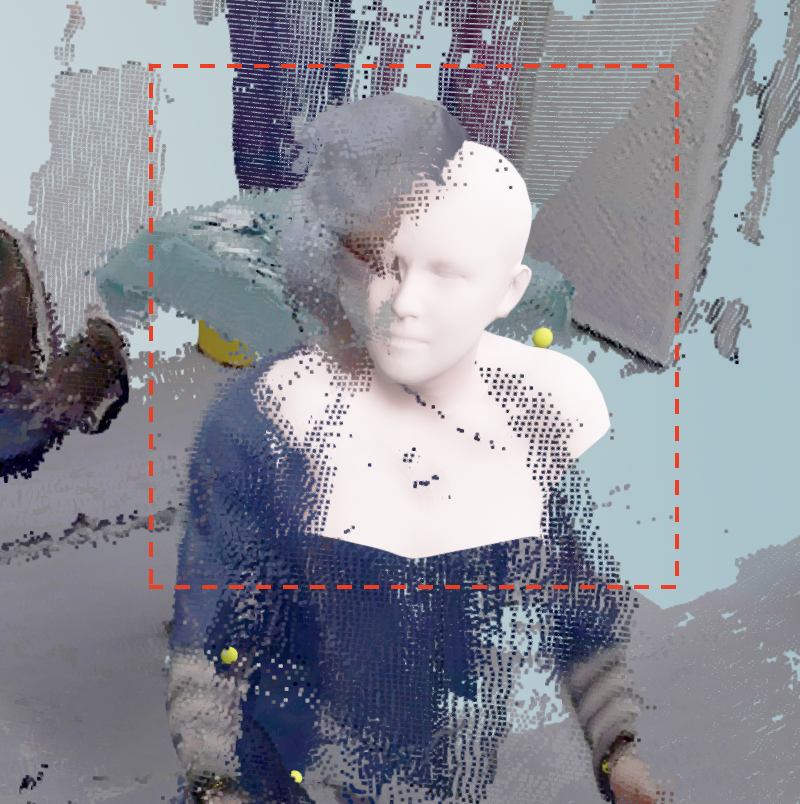
\includegraphics[width=0.65\columnwidth]{figures/issue_pointcloud.png}
    \caption{The upper body of an estimated parametric human mesh model with the point cloud. For a rigid registration it would be necessary to extract the head of the mesh.}
    \label{fig:example_mesh}
\end{figure}

\subsection{Dataset}
The data used in Bastian and Wang et al.~\cite{disguisor} is still undisclosed, hence we perform our experiments on different data.
The data we use was acquired from the chair of Computer Aided Medical Procedures (CAMP) at TUM (Fig.~\ref{fig:example_pcd}) by capturing a simulated OR environment from six calibrated ceiling-mounted Microsoft Azure Kinect cameras.
Each frame consists of six RGB images and a fused point cloud of the scene.

\begin{figure}[!ht]
    \centering
    \includegraphics[width=\textwidth]{figures/point_cloud.png}
    \caption{Example of a point cloud from our dataset we use for evaluation.}
    \label{fig:example_pcd}
\end{figure}

\subsection{Methods}

\textbf{Training} The authors of DCP~\cite{dcp} already published their code base on GitHub\footnote{https://github.com/WangYueFt/dcp}.
We will first use their pre-trained model and compare their method qualitatively against existing methods like FilterReg~\cite{filterreg} and ICP~\cite{icp}.
Subsequently, we extend the ModelNet 40~\cite{modelnet40} dataset to adapt it to our use case.
Apart from augmenting the ModelNet 40 dataset by mirroring real life data (noise and sparseness), we add synthetic data that resembles our use case.
More specifically, we generate a synthetic dataset by sampling different human poses using the parametric human mesh model SMPL~\cite{SMPL:2015} and converting it to a point cloud. 
We copy the head, apply a random transformation to it and perform several augmentations on the original SMPL model point cloud.

\noindent\textbf{Evaluation}
We will evaluate our approach qualitatively.
Evaluating our approach quantitatively might become difficult, as there is no ground truth data available for our dataset.
Moreover, generating ground truth is not trivial, as transformations can be ambiguous if the point cloud is incomplete.
We could, however, evaluate our approach quantitatively using the method introduced in Bastian and Wang et al.~\cite{disguisor} by annotating face bounding boxes in the 2D images and rendering the head meshes back into the 2D images.

% List your requirements, e.g. dataset, which type of data you need for your approach (SDF, point clouds, etc.) and how you will generate them from the dataset you want to use.

\section{Team}
Tony Wang 03726379

% references
{\small
	\bibliographystyle{plain}
	\bibliography{bibliography}
}

\end{document}